

\usetikzlibrary{patterns}
\begin{figure}[t!]
\begin{center}
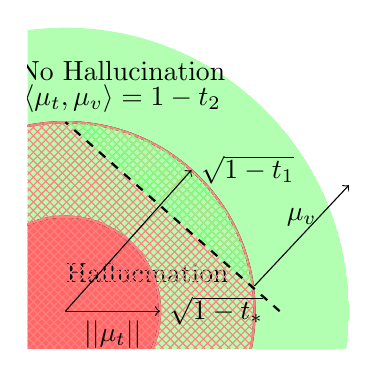
\begin{tikzpicture}[scale=.8]
    % Clip to only the positive quadrant
    \clip (-0.6,-0.6) rectangle (4.5,4.5);
    
    % Outer background circle (larger than radius 3)
    \begin{scope}
      \clip (0,0) circle (4.5);
      \fill[green!30] (0,0) circle (4.5);
    \end{scope}
    
    % Inner hallucination circle
    \fill[red!60] (0,0) circle (1.5);
    \draw[thick] (0,0) circle (1.5);
    \node at (1.3,0.6) {Hallucination};
    
    % Outer decision boundary circle
    \draw[thick] (0,0) circle (3);
    \draw[thick,red!50,pattern=crosshatch,pattern color=red!50] (0,0) circle (1.5) (0,0) circle (3);
    
    % Green crosshatched area (no hallucination region)
    \begin{scope}
        \clip (0,0) circle (3);
        \clip (3.4,0) -- (0,3) -- (4,3.7) -- (3,3.7) -- cycle;
        \draw[thick,green!50,pattern=crosshatch,pattern color=green!50] (5,0) rectangle (0,5);
    \end{scope}
    
    % Vectors and labels
    \draw[->] (0,0) -- (1.5,0) node[midway, below] {$||\mu_t||$};
    \node[right] at (1.5,0) {$\sqrt{1-t_*}$};
    
    \draw[->] (0,0) -- (2,2.24);
    \node[right] at (2,2.24) {$\sqrt{1-t_1}$};
    
    \draw[thick, dashed] (3.4,0) -- (0,3);
    \node[above] at (0.9,3) {$\langle \mu_t, \mu_v \rangle = 1 - t_2$};
     \node[above] at (0.9,3.5) {No Hallucination};
    
    \draw[->] (3,0.4) -- (4.5,2) node[midway, above] {$\mu_v$};
    
    % Equations
   % \node at (1.9,-0.5) {$\|\mu_t \|^2 = 1 - \mpd(\mself)$};
   % \node at (1.9,-1) {$\langle \mu_t,\mu_v \rangle= 1 - \mpd(\mcross)$};    
\end{tikzpicture}
\end{center}
\vspace{-.2cm}
\caption{Geometric interpretation in mean embeddings spaces of ``target" ($\mu_t$) and ``verifier" distributions ($\mu_v$). Self consistency is measured via the norm of mean embeddings of the target model, and cross consistency via the dot product between mean embeddings. In stage one, detection is based on $\|\mu_t\|$, and we have no hallucination outside the sphere of radius $\sqrt{1-t_1}$ (in green) and hallucination within the sphere of radius $\sqrt{1-t_*}$ (in red). Between the two sphere the hyperplane defined by $\mu_v$ and $t_2$, splits this area in two zones: above it for no hallucination (dashed green) and below it for hallucination (dashed red).   }
\label{fig:geometry}
\vspace{-.2cm}
\end{figure}

\textbf{Geometric Interpretation in Mean Embedding Space.} We provide a geometric interpretation of our hallucination detection. 
For each prompt $x$ we can observe the conditional distribution of the target model  $\pi_t(y|x)$ and the verifier $\pi_v(y|x)$. In particular we observe $ \frac{1}{n_a} \sum_{i=1}^{n_a} \delta_{y^a_i},$ $y^a_i\sim \pi_t(.|x)$ and $ \frac{1}{n_v} \sum_{i=1}^{n_v} \delta_{y^v_i},y^v_i\sim \pi_v(.|x)$. We assume that the entailment kernel $\mathcal{E}: \mathcal{Y} \times\mathcal{Y} \to [0,1]$ to be a reproducing kernel. The mean embeddings \cite{Muandet_2017} of target, verifier and ground truth are respectively
$ \mu_t = \frac{1}{n_a} \sum_{i=1}^{n_a} \mathcal{E} (y^a_i,.)$,
$\mu_v = \frac{1}{n_v} \sum_{i=1}^{n_v} \mathcal{E} (y^v_i,.),$ and $\mu^* = \frac{1}{n^*} \sum_{i=1}^{n^*}\mathcal{E}(y^*_i, .)$ We can write the self-consistency in terms of norms of mean embeddings : 
\[\| \mu_t\|^2 = \frac{1}{n_a^2}\sum_{i,j} \mathcal{E}(y^a_i, y^a_j) =  1 - \mpd(\mself)\]
and the cross-consistency
\[\langle 
\mu_t,\mu_v\rangle = \frac{1}{n_an_v}\sum_{i,j} \mathcal{E}(y^a_i, y^v_j) = 1-\mpd(\mcross)\]
%Note that  we assume that there exists a threshold $\tau$  such that $ ||\mu^*||^2 \geq \tau$ almost surely for $x$. 
Fig. \ref{fig:geometry} gives a geometric interpretation of our two stage algorithm in means embedding spaces. If the ``target" model norm of mean embedding is higher than a treshold $\sqrt{1-t_1}$  no hallucination is detected   and for a norm less than a treshold $\sqrt{1-t^*}$ is detected. For the uncertainty area between the two spheres, the verifier mean embedding defines with the treshold $1-t_2$ a hyperplane that divides this area in no hallucination (above) and hallucination (below).  




% We analyze here the combination of self and cross consistency discussed in Section \ref{sec:weighting}. The following proposition shows that the optimal combination of target and verifier corresponds to a weighting that emphasizes the most accurate one with respect to ground truth. 
% \begin{proposition}
% The optimal weight $\lambda$ for combining self and cross consistencies to approximate the consistency of the target with the ground truth satisfies:
% $\min_{\lambda \in [0,1]}| \langle\mu_t, \lambda \mu_t + (1-\lambda) \mu_v\rangle - \langle\mu_t,\mu^*\rangle | \leq \min_{\lambda \in [0,1]} \sqrt{2(1-\langle\mu_*, \lambda \mu_t + (1-\lambda) \mu_v\rangle )}.$
% Hence it is enough to solve:
% $ \max_{\lambda \in [0,1]} \langle\mu_*, \lambda \mu_t + (1-\lambda) \mu_v\rangle$. Using an entropic regularization  of this objective  for $\varepsilon>0$: $\max_{\omega_t,\omega_v \in [0,1],\omega_t+\omega_v=1} \langle\mu_*, \omega_t \mu_t + \omega_v \mu_v\rangle - \varepsilon (\sum_{j\in \{t,v\}} \omega_j (\log \omega_j-1) ,$ we obtain $\lambda^*= \frac{\exp(\frac{\langle \mu_t, \mu^*\rangle}{\varepsilon})}{\exp(\frac{\langle \mu_t, \mu^*\rangle}{\varepsilon})+ \exp(\frac{\langle \mu_v, \mu^*\rangle}{\varepsilon}) }.$ 
% \end{proposition}


% \subsection{ROC generalization}
% \kg{This can go after wherever we define the threshold selection procedure}

\textbf{Evaluating AUROC/AURAC for Algorithm \ref{alg: two_stage}.} Recall that, in the conventional scenario, the AUROC and AURAC metrics are defined for a system that outputs a single value for binary classification. To compute these metrics, we vary the threshold used to produce the label from the output. In such cases, for both ROC and RAC curves, each $X$-value corresponds to a single $Y$-value. For example, in ROC, one false positive rate corresponds to one true positive rate, allowing us to obtain a single curve by varying the threshold and then compute the area under it. However, the situation is more complex for our Algorithm \ref{alg: two_stage}, which, given a fixed hyperparameter $p$, ultimately outputs binary labels but involves two thresholds, $t_1$ and $t_2$. Different combinations of $t_1$ and $t_2$ can yield the same $X$-value but different $Y$-values, resulting in a plot that resembles a thick band rather than a single curve. Thus, the area under the curve is not well-defined. The way these thresholds are adjusted relative to each other significantly affects the $Y$ values for a given $X$. To derive a meaningful performance measure for our algorithm, we establish the relationship between the two thresholds using a validation set. Specifically, on this set, we iterate over a grid of threshold combinations, running the algorithm to obtain all $X,Y$ pairs. For each small interval of $X$, we identify the threshold combinations that maximize $Y$. Next, we use a separate test set, where we only evaluate the good combinations identified from the validation step and compute the resulting AUROC/AURAC. We note that prior work \cite{lin2023generating,nikitin2024kernel} also relies on a validation set for tuning hyperparameters. 

We now prove that the above procedure for selecting the two thresholds from data achieves a test-time AUROC close to the optimal value achieved on the validation set. Our theorem below applies more generally to any method that uses data to select from a finite set of threshold values.
%\vspace{-.2cm}
\begin{theorem}[AUROC Generalization]\label{thm:ROC}
Suppose we are given $n_{neg}$ i.i.d. samples from the non-hallucinating distribution and $n_{pos}$ i.i.d. samples from the hallucinating distribution, and  sets of candidate thresholds $\mathcal{T}_1 = \{t^1_j\}_{j=1}^{|\mathcal{T}_1|}$ and $\mathcal{T}_2 = \{t^2_k\}_{k=1}^{|\mathcal{T}_2|}$ for stages 1 and 2 respectively. Suppose we use this data to choose a mapping $t_1,t_2 = \mathcal{A}(p_{FA})$ from desired probability of false alarm level $p_{FA}\in [0,1]$ to thresholds $t_1 \in \mathcal{T}_1, t_2 \in \mathcal{T}_2$, maximizing the probability of detection on the validation data. Let $A_{val}(\mathcal{A})$ be the AUROC using thresholds given by $\mathcal{A}$. Then, with probability at least $\left(1 - \frac{2}{|\mathcal{T}_1| |\mathcal{T}_2|}\right)^2$, the test AUROC satisfies
$
A_{test}(\mathcal{A}) \geq A_{val}(\mathcal{A}) - 2\epsilon$
and the test $|p^{test}_{FA} - p_{FA}| \leq \epsilon$, where
$
\epsilon = \sqrt{\frac{\log(|\mathcal{T}_1|) + \log(|\mathcal{T}_2|)}{\min(n_{neg}, n_{pos})}}$.
\end{theorem}
\vspace{-.2cm}

The proof is in Appendix \ref{app:ROC}.
Note that this theorem implies we need to have $
\mathrm{n_{neg}}, \mathrm{n_{pos}} = \Omega\left(\log(|\mathcal{T}_1|) + \log(|\mathcal{T}_2|)\right)$ to guarantee the test AUROC is close to the convex-hull-AUROC on validation data. Furthermore, in Section \ref{sec: exp}, we validate through experiments that the selected thresholds transfer well to the test data.\looseness=-1

